%%=============================================================================
%% Resultaten
%%=============================================================================

\chapter{\IfLanguageName{dutch}{Resultaten}{Results}}
\label{ch:resultaten}

\section{Resultaten van de data die verzameld is}
Via het formulier van ``JotForm'' waren er 13 inzendingen. Dat lijkt niet veel, maar er moet wel geweten zijn dat dit niet zomaar snel een vragenlijst invullen is. Er werd telkens gevraagd om een eigenschappen van \textit{elderspeak} na te bootsen door een geluidsfragment in te spreken. Dit is veel meer werk waardoor mensen sneller afhaakten.

Toch gaven deze 13 personen 54 audiobestanden ter beschikking. Op die geluidsbestanden kon er gecontroleerd worden of er \textit{elderspeak} aanwezig bij was.

De data is gelabeld door een persoon, dus het kan zijn dat er fouten in de classificatie van de data zit. Dit eindwerk is natuurlijk een van de richting toegepaste informatica, en niet van een communicatierichting. Een interessante opdracht kan dan zijn dat er een interdisciplinaire opdracht komt waarbij studenten verpleegkunde of communicatie nieuwe data labelen en studenten toegepaste informatica testen uitvoeren op de server.

Meer hierover wordt beschreven in het vervolg verhaal, namelijk Hoofdstuk~\ref{ch:vervolg}.

\section{Resultaten na het testen}
De testen worden weergegeven in een \textit{confusion matrix}. Daarbij is te zien dat er op de x-as de echte waarden staan, waarbij de echte waarden gelijk staan aan de waarden die gegeven werden bij het labelen van de data. De waarden op de y-as zijn de voorspelde waarden van de applicatie (\textit{back-end} of berekeningen).

\subsection{Verkleinwoorden}
De testgevallen van de verkleinwoorden zijn te vinden in \textit{confusion matrix}~\ref{fig:cfm_verkleinwoord}. Daarbij is te zien dat er 8 correcte positieven zijn, 3 vals positieven, 5 valse negatieve en 38 correct negatieven.
Hieruit kunnen we afleiden dat de applicatie goed de verkleinwoorden weet te vinden.
\begin{figure}
	\centering
	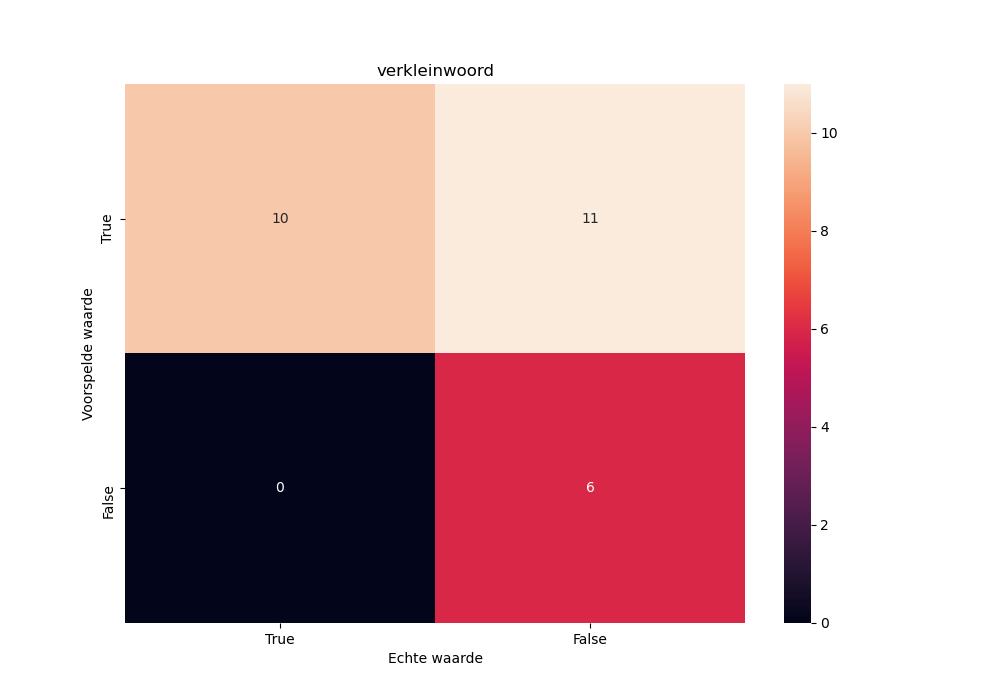
\includegraphics[width=1\textwidth]{./img/cfm_verkleinwoord}
	\caption{\label{fig:cfm_verkleinwoord} Resultaten \textit{confusion matrix} verkleinwoorden}
\end{figure}


\subsection{Toonhoogte}
De \textit{confusion matrix} van de testgevallen van de toonhoogte is te vinden in figuur~\ref{fig:cfm_pitch}. Daar is te zien dat er 5 correcte positieven zijn, 10 vals positieven, 7 valse negatieve en 32 correctie negatieven.
Hieruit kunnen we afleiden dat de applicatie een beetje werkt voor de toonhoogte, maar dat hij er soms wel naast durft te zitten.
\begin{figure}
	\centering
	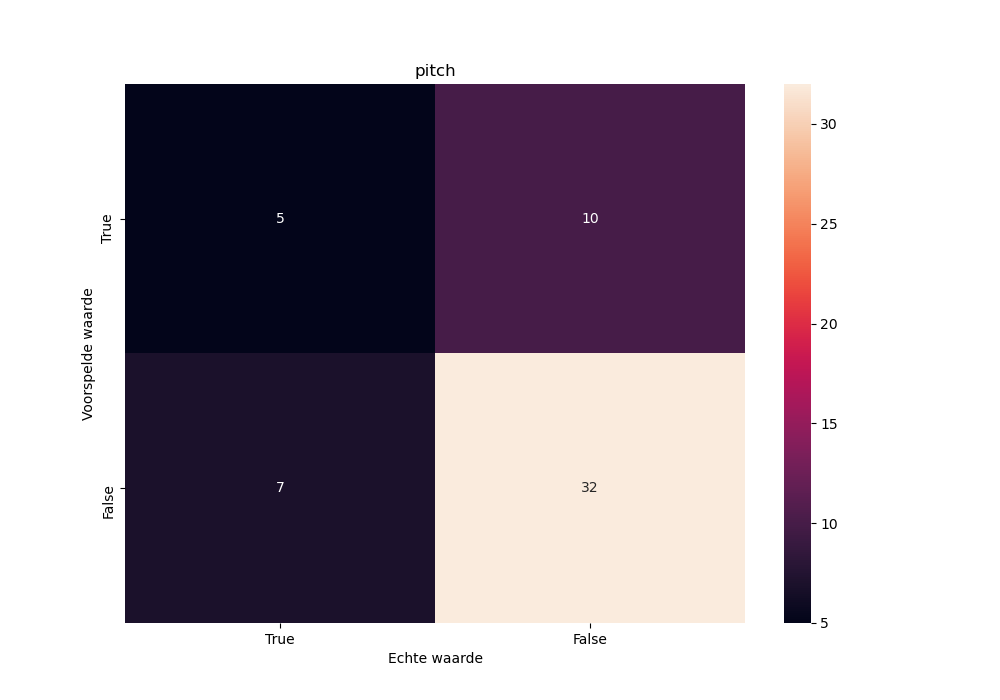
\includegraphics[width=1\textwidth]{./img/cfm_pitch}
	\caption{\label{fig:cfm_pitch} Resultaten \textit{confusion matrix} toonhoogte}
\end{figure}

\subsection{Stemvolume}

De \textit{confusion matrix} van de testgevallen van het stemvolume is te vinden in figuur~\ref{fig:cfm_pitch}. Daar is te zien dat er 4 correcte positieven zijn, 2 vals positieven, 4 valse negatieve en 44 correctie negatieven.
Hieruit kunnen we afleiden dat de applicatie wel goed werkt, maar toch een zekere foutenmarge heeft.
\begin{figure}
	\centering
	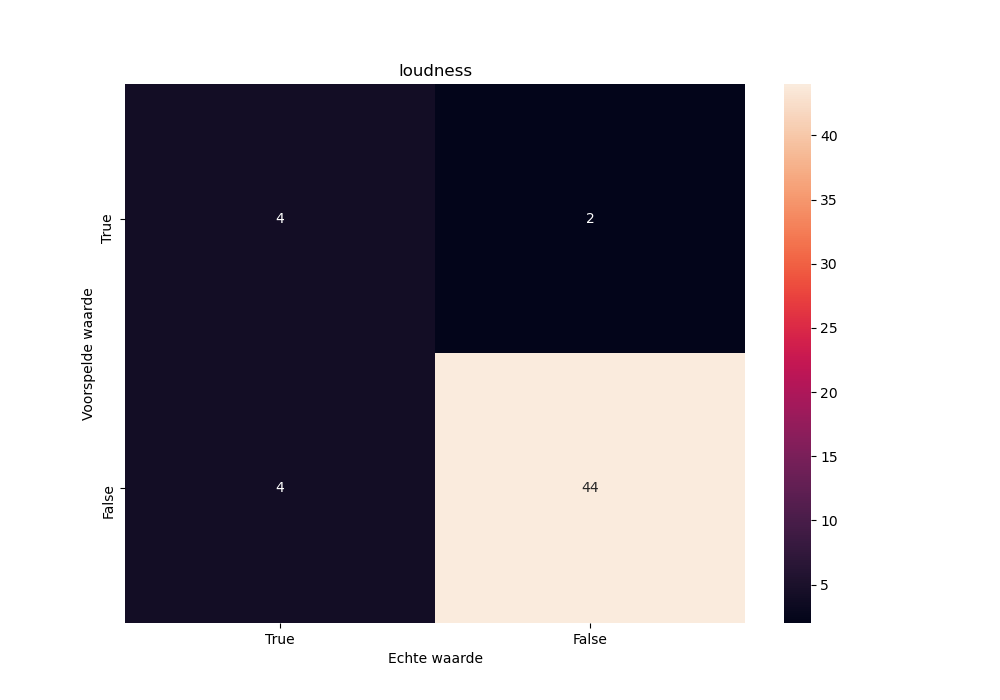
\includegraphics[width=1\textwidth]{./img/cfm_loudness}
	\caption{\label{fig:cfm_loudness} Resultaten \textit{confusion matrix} stemvolume}
\end{figure}

\subsection{Algemeen besluit na testen}
We kunnen wel goed zien a.d.h.v. deze \textit{confusion matrixes} dat er te weinig testgevallen zijn om een mooi beeld te vormen of de applicatie werkt. We moeten meer gevallen verzamelen waarbij de toonhoogte of stemvolume hoger zijn en waarbij er verkleinwoorden aanwezig zijn.

\section{Rollenspel}
Wanneer er een rollenspel gespeeld wordt, dan wordt de audio van beide personen geanalyseerd. Het is niet direct mogelijk om een stem weg te filteren als beide personen aanwezig zijn in de kamer. Alleen wanneer een van de twee personen significant verder staan van de microfoon, zal de applicatie die stem kunnen wegfilteren als achtergrondlawaai.

Toch kan er nog steeds geanalyseerd worden of er \textit{secondary baby talk} aanwezig is, dus de applicatie kan gebruikt worden om conversaties te oefenen.

\section{Zijn de \textit{requirements} voldaan?}
De \textit{requirements} zijn weldegelijk voldaan. Zo kan de applicatie de \textit{elderspeak} detecteren, weliswaar met een foutenmarge die te lezen is in de resultaten na het testen.
Daarnaast is de webapplicatie te draaien op een computer en is alles in een mooie lay-out gegoten.
Zo waren de applicatie en de paper meer dan genoeg op tijd klaar. Daarnaast is er ook een vervolg hoofdstuk geschreven in Hoofdstuk~\ref{ch:vervolg} zodat dit onderzoek niet voor niets was.
